\chapter{Stato dell'arte}
\label{ch:stato_arte}

%%%%%%%%%%%%%%%%%%%%%%%%%%%%%%% Introduzione Internet of Things
% https://www.internet4things.it/iot-library/internet-of-things-gli-ambiti-applicativi-in-italia/
% https://www.robotiko.it/linternet-delle-cos-e-definizione-esempi/
% https://www.avsystem.com/blog/what-is-internet-of-things-explanation/
\section{Internet of Things}
L'Internet of Things (IoT) \cite{atzori2010internet} è un paradigma che ha guadagnato rapidamente notorietà nello scenario delle telecomunicazioni wireless. Può essere definito come un neologismo utilizzato nel campo delle telecomunicazioni, nato dall'esigenza di dare un nome agli oggetti reali connessi ad Internet. Attraverso schemi di indirizzamento unici, questi dispositivi sono in grado di interagire e cooperare con i propri vicini al fine di raggiungere obiettivi comuni.
Nel concreto, con Internet of Things \cite{li2015internet, rose2015internet} indichiamo un insieme di tecnologie che permettono di collegare alla rete Internet qualunque tipo di apparato che ci circonda. Tali apparati raccolgono e si scambiano dati in tempo reale, comunicano il proprio status e inviano dati sul proprio operato, accedono ad informazioni utili per il proprio funzionamento in modo del tutto automatico. Esse sono anche in grado di comunicare con il mondo esterno e di fornire informazioni alle quali prima non avevamo accesso. \\
Lo scopo preposto da queste tecnologie prevede l'attività di monitoraggio e controllo dell'ambiente circostante e il trasferimento di dati per poi svolgere azioni conseguenti.\\
Apparecchi e dispositivi con queste caratteristiche sono definiti \textit{smart object} (oggetti ``intelligenti') ed offrono la possibilità di unire il mondo reale con quello virtuale.\\

\noindent Sebbene l'IoT si sia diffuso nell'ultimo decennio, Nikola Tesla, un famoso visionario serbo, aveva già previsto la sua ascesa nella rivista Collier nel 1926: ``\textit{... quando la tecnologia wireless verrà applicata perfettamente, l'intera terra verrà convertita in un enorme cervello [...] e gli strumenti attraverso i quali saremo in grado di farlo saranno incredibilmente semplici rispetto ai telefoni attuali. Un uomo sarà in grado di portarne uno nella tasca della giacca}'' \cite{kennedy1926woman}.\\
Il termine ``Internet of Things'' (IoT) è usato per la prima volta nel 1999 dal pioniere della tecnologia, l'ingegnere inglese Kevin Ashton - direttore esecutivo dell'Auto-ID Center, un'organizzazione di ricerca globale, indipendente e non profit, con sede presso il MIT (Massachusetts Institute of Technology) - per descrivere un sistema costituito da oggetti presenti nel mondo reale (mondo fisico) in grado di acquisire una propria identità nel mondo digitale, attraverso la capacità di connettersi ad internet. Ashton coniò il termine per illustrare l'utilizzo della tecnologia Radio-Frequency Identification (RFID) nella filiera aziendale al fine di tener traccia dei beni senza necessità dell'intervento umano.\\

\noindent I quattro elementi indispensabili per l'Internet of Things: 
\begin{itemize}
    \item con il termine \textit{Things} indichiamo qualsiasi oggetto che possiamo collegare ad Internet. I compiti delle smart things includono non solo la raccolta dati, ma anche la comunicazione con le altre things, con server remoti o con il cloud ed eseguire azioni basate sui comandi ricevuti.
    
    \item la \textit{Connettività} comprende tutto ciò che consente di avere una comunicazione tra gli smart object. Il linguaggio è rappresentato dai protocolli specifici dell'IoT, il canale di comunicazione è assicurato dalle note soluzioni di connettività come Wi-Fi, Bluetooth, etc. L'adozione di una soluzione piuttosto che un'altra dipende in gran parte dai requisiti e dai limiti dello specifico progetto IoT, dal momento che tutte le forme di connettività rappresentano un compromesso tra consumo energetico, range di copertura e ampiezza di banda. 
    
    \item con il termine \textit{Software} indichiamo tutte quelle istruzioni che consentono ai dispositivi di eseguire compiti specifici, come raccogliere dati in modo strutturato, analizzarli, gestirli, etc. Sulla base dei dati acquisiti è il software che decide se devono essere intraprese azioni o se ad esempio l'utente deve essere informato tramite un alert.
    
    \item il livello \textit{Applicativo} fa sì che l'utente possa interagire con gli oggetti, ma consente anche di visualizzare informazioni utili sul funzionamento dell'intero sistema. 
\end{itemize}

% https://blog.osservatori.net/it_it/cos-e-internet-of-things
% https://www.zerounoweb.it/analytics/big-data/internet-of-things-iot-come-funziona/
\noindent L’Internet of Things \cite{minteer2017analytics} è un paradigma che non conosce, potenzialmente, confini applicativi: dall’autovettura che dialoga con l’infrastruttura stradale per prevenire incidenti, agli elettrodomestici di casa che si coordinano per ottimizzare l’impiego di potenza; dagli impianti di produzione che scambiano dati con i manufatti per la gestione del loro ciclo di vita ai dispositivi medici che si localizzano nel presidio di un pronto soccorso, persino agli sci che inviano informazioni sullo stato della neve, o sulla severità di una caduta. Se è vero che tutti gli oggetti possono diventare “intelligenti” connettendosi alla rete e scambiando informazioni su di sé e sull’ambiente circostante, è altrettanto vero che questo processo non avviene in tutti gli ambiti con la stessa velocità: ciò dipende dall’esistenza di soluzioni tecnologiche consolidate, dagli equilibri competitivi in un determinato mercato e, in definitiva, dal bilancio tra il valore dell’informazione e il costo di creazione della rete di oggetti intelligenti.\\

\noindent Si possono definire diversi ambiti applicativi dell'Internet of Things \cite{marjani2017big}, alcuni di essi sono riportati di seguito.
\begin{itemize}
    \item \textit{Smart Agriculture}: prevede il monitoraggio di parametri microclimatici a supporto dell'agricoltura per migliorare la qualità dei prodotti, ridurre le risorse e l'impatto ambientale.
    
    \item \textit{Smart Car}: prevede delle auto (connesse) in grado di comunicare con l'ambiente circostante. Sono in grado di connettersi con altri veicoli o con l'infrastruttura circostante per la prevenzione e la rivelazione di incidenti, traffico, etc. Oltre a connettere i veicoli tra loro, l'IoT in questo campo consente il controllo remoto della posizione e lo stato di funzionamento del veicolo, la protezione degli occupanti in caso di incidente con l'immediata comunicazione ai servizi sanitari e assicurati e persino la gestione del noleggio del veicolo.
    
    \item \textit{Smart City}: monitoraggio e gestione degli elementi di una città (ad esempio mezzi per il trasporto pubblico, illuminazione pubblica e parcheggi) e dell’ambiente circostante per migliorarne vivibilità, sostenibilità e competitività.
    
    \item \textit{Smart Home}: soluzioni per la gestione in automatico e/o da remoto degli impianti e degli oggetti connessi dell’abitazione, con il fine di ridurre i consumi energetici e migliorare il comfort, la sicurezza dell’abitazione e delle persone al suo interno.
    
    \item \textit{Smart Metering}: contatori connessi (Smart Meter) per la misura dei consumi (elettricità, gas, acqua, calore), la loro corretta fatturazione e la tele-gestione.
    
    \item \textit{Smart Industry}: connessione dei macchinari, degli operatori e dei prodotti per abilitare nuove logiche di gestione della produzione. Con ciò è possibile rendere intelligenti macchine e linee di produzione, consentendo l'elaborazione in tempo reale e quindi l'avvio di processi automatici e allarmi. L'informazione generata attraverso questi processi e la capacità di controllo consentono previsioni più attendibili, benefici a livello della flessibilità e del bilancio energetico, riduzione degli scarti, oltre al monitoraggio dell'elaborato in ogni fase della produzione.
\end{itemize}

\noindent I dispositivi terminali che appartengono a questo immenso mondo dell'IoT solitamente hanno i seguenti requisiti: piccole dimensioni, bassa potenza e spesso alimentati a batteria. Un tipico esempio sono i sensori e attuatori impiegati nella quotidianità, in cui la resilienza, la robustezza nella comunicazione e un ridotto consumo energetico sono fondamentali per il loro successo.

% http://www.intelligenzaartificiale.it/internet-of-things/#Internet_of_Things_IoT_o_Internet_delle_cose_cos8217e
% \noindent La diffusione sempre più capillare, già in atto, di oggetti collegati alla rete al di fuori del controllo dei suoi proprietari ha già innescato diverse polemiche e controversie.  Innanzitutto, si è preoccupati per il rispetto della \textit{privacy}: se gli oggetti di uso comune sono collegati in rete è teoricamente possibile raccogliere un'infinità di dati sulle abitudini dei singoli in ogni ambito.\\ La dispersione di dati è sempre una possibilità e questo ha posto l'attenzione sul problema della \textit{sicurezza}.  La necessità è quella non solo di gestire i big data così raccolti, ma anche di far fronte alla possibilità che attacchi informatici immobilizzino una parte sempre più consistente della vita quotidiana, come bloccare il traffico automobilistico, la produzione industriale, i riscaldamenti nelle case e lasciare senza energia elettrica e assistenza i pazienti degli ospedali.

%%%%%%%%%%%%%%%%%%%%%%%%%%%%%%% Machine to machine
% https://www.internet4things.it/m2m/machine-to-machine-m2m-cose-come-funziona-e-a-cosa-serve/
% https://www.avsystem.com/blog/iot-and-m2m-what-is-the-difference/

\section{Machine-to-Machine}
La tecnologia Machine-to-Machine (M2M) deriva da quella della telemetria e può essere descritta come \textit{``l'insieme di algoritmi e procedure che consentono a dei sistemi embedded di poter svolgere in maniera autonoma delle operazioni in funzione del trasferimento dei dati da un dispositivo all'altro tramite reti cellulari o cablate senza che ci sia alcun intervento da parte dell'uomo o che questo possa essere in percentuale molto bassa o irrisoria''} \cite{m2m}.\\
M2M è stato utilizzato nel corso dei decenni come tecnologia standard nella telemetria, ancor prima dell'avvento dell'IoT, poiché prevedeva una semplice interazione tra due o più macchine senza la partecipazione umana.\\
Per parlare di M2M, come lo intendiamo oggigiorno, si è dovuto aspettare la miniaturizzazione dei componenti, lo sviluppo di protocolli di comunicazione comuni e delle reti dati (wireless e telefonica), ma soprattutto la definizione degli standard.\\

\noindent Questa tecnologia consente di integrare e far dialogare delle apparecchiature (anche di tipologia diversa) installate a qualunque distanza tra loro attraverso dei sensori che inviano (o acquisiscono) dati per poi trasmetterli ad un server centrale tramite una rete. 
I sistemi M2M utilizzano nella maggior parte dei casi reti wireless, dove si devono avere come minimo due dispositivi muniti di sensori, un collegamento di comunicazione attraverso protocolli comuni e un software di calcolo autonomo. Questo software è specificatamente programmato per far si che un dispositivo di rete possa interpretare i dati e prendere quindi le adeguate decisioni.\\
Le applicazioni M2M acquisiscono i dati, i quali possono attivare azioni automatizzate sui dispositivi embedded. Tale soluzione è particolarmente importante in ambito industriale dove la comunicazione da remoto, tra macchinari e dispositivi, deve avvenire in maniera coordinata per la realizzazione di un determinato obiettivo programmato, in modo da poter rendere efficiente la produzione e l’intero ciclo operativo.\\

\noindent % Il range di queste tecnologie è limitato a poche centinaia di metri al massimo. 
L'area di copertura di queste tecnologie può essere tranquillamente ampliata utilizzando una fitta rete di dispositivi e gateway connessi mediante reti mesh multi-hop. Di contro, la creazione di una rete di grandi dimensioni risulta essere proibitivamente costosa.

% DA RIVEDERE __________ RIMOSSA
% \noindent Esistono differenze sostanziali tra la tecnologia Machine to Machine e Internet of Things (IoT). Formalmente M2M e IoT fanno la stessa cosa (comunicazione tra dispositivi connessi), ma nella prima le singole apparecchiature sono collegate in rete in un sistema chiuso, l'IoT, invece, consente di collegare più sottosistemi di M2M in un sistema che interagisce con l'ambiente fisico (smart object) e con le persone.\\
% I sistemi basati su M2M utilizzano trasmissioni point-to-point tra dispositivi, con sensori e hardware dedicato, comunicanti tramite reti cellulari o sistemi chiusi (wireless o wired), mentre i sistemi IoT operano attraverso reti basate su protocollo IP per inviare e gestire i dati raccolti da apparati di rete specifici quali gateway, middleware o piattaforme cloud.

%%%%%%%%%%%%%%%%%%%%%%%%%%%%%%% Communication
% INTRO to Bluetooth Low Energy
\section{Wireless Personal Area Network}
Una Wireless Personal Area Network (WPAN) è l'interconnessione di dispositivi informatici con un raggio di comunicazione relativamente ridotto, in genere di circa 10 metri, in cui le connessioni sono di natura wireless. Ciò consente l'impiego di piccoli dispositivi efficienti dal punto di vista energetico ed economico.\\
La comunicazione tra tali dispositivi è basata sul concetto architetturale di livelli, dove quelli inferiori non necessariamente devono conoscere quelli al di sopra. Esiste un'ampia varietà di protocolli di rete sia per la connettività dei dispositivi sia per la comunicazione dei dati generati da essi. Il protocollo adoperato dipende dal tipo di dispositivo e dal tipo di ambiente in cui esso è collocato.\\
La connettività è fondamentale, poiché stabilisce un metodo per comunicare tra due o più apparati. Le strategie utilizzate sono influenzate dai vincoli dei dispositivi e il consumo energetico è spesso il più significativo.\\

\noindent Gli standard coinvolti nelle WPAN comprendono le comunicazioni infrarossi (IrDA), le due varianti Bluetooth (BR/EDR e BLE) e le tecnologie basate sullo standard 802.15.4 (definisce sia il livello fisico che il livello di collegamento del modello OSI), come 6LoWPAN, ZigBee.\\
Le tecnologie Bluetooth Low Energy, 6LoWPAN, ZigBee sono orientate a privilegiare il risparmio energetico piuttosto che avere un elevato tasso di trasferimento dati. Il Wi-Fi, invece, è una tecnologia orientata a massimizzare il trasferimento dei dati, garantendo una velocità e un bit-rate maggiore rispetto alle tecnologie precedenti. A tal proposito richiede una maggiore complessità nei dispositivi e soprattutto comporta maggiori consumi energetici.

\subsubsection{802.15.4}
L'Institute of Electrical and Electronics Engineers (IEEE) ha rilasciato nel 2003 lo standard 802.15.4 per regolamentare le Low Power Wireless Personal Area Network (LP-WAN), fornendo il primo standard globale per le comunicazioni radio a bassa potenza  \cite{callaway2002home}.
Tale standard definisce le specifiche dei primi due livelli dello stack protocollare, ovvero il livello Fisico (PHY) e il livello di collegamento (MAC), senza specificare nessun requisito per i livelli superiori, a discrezione delle singole applicazioni.
A tal proposito, protocolli come ZigBee e 6LoWPAN definiscono delle proprie caratteristiche per i livelli di rete, di applicazione e anche in merito alla sicurezza, mentre per i primi due livelli adottano i requisiti definiti dallo standard LP-WAN.\\

\noindent Lo standard 802.15.4 consente di classificare i dispositivi appartenenti ad una wireless network in due categorie principali: \textit{full-function devices} (FFD) e \textit{reduced-function devices} (RFD). I dispositivi FFD sono in grado di eseguire tutti i compiti descritti dallo standard come, creazione della rete, processo di routing, gestione della rete, quindi sono in grado di ricoprire qualsiasi ruolo all'interno della rete. I dispositivi RFD, d'altra parte, hanno capacità limitate, essi, infatti, sono destinati ad applicazioni molto semplici come l'accensione o lo spegnimento di un interruttore. I dispositivi FFD possono comunicare con qualsiasi altro dispositivo in una rete, mentre gli RFD possono dialogare solo con dispositivi FFD. Un'altra caratteristica che contraddistingue le due categorie riguarda la capacità di elaborazione e la dimensione della memoria, normalmente inferiore per quanto riguarda gli RFD.\\
Un dispositivo FFD può ricoprire uno qualsiasi dei tre differenti ruoli presenti in una rete 802.15.4: \textit{coordinator}, \textit{PAN coordinator}, e \textit{device}. Il ruolo del Coordinatore riguarda l'inoltro dei messaggi e se il dispositivo, ha anche il compito di gestire l'intera rete, ossia una Personal Area Network (PAN), è definito PAN coordinator. Nel caso in cui un dispositivo non agisce da coordinatore è semplicemente un device. Quest'ultimo è l'unico ruolo ricopribile da entrambe le tipologie, FFD e RFD.\\

\noindent In merito alla comunicazione, IEEE 802.15.4, implementa un metodo semplice per consentire a più dispositivi di adoperare lo stesso canale di frequenza per comunicare. Ci sono due modalità di funzionamento, una denominata \textit{beacon-enabled} e l'altra \textit{non-beacon enabled}. Entrambe le modalità gestiscono l'accesso al canale trasmissivo utilizzando il protocollo \textit{Carrier Sense Multiple Access with Collision Avoidance} (CSMA-CA). Nello specifico nella modalità beacon-enabled viene utilizzato uno Slotted CSMA-CA, mentre nella modalità non-beacon-enabled si usa l'unslotted o standard CSMA-CA.\\

\noindent La modalità \textit{beacon-enabled} è chiamata anche modalità strutturata e gestisce la comunicazione attraverso l'uso di un apposito messaggio, denominato \textit{beacon}. Questo messaggio prevede un formato specifico ed è usato per sincronizzare il clock dei nodi appartenenti alla rete, definendo una finestra temporale, \textit{superframe}, per regolamentare l'accesso al canale. All'interno dell'intervallo vengono definiti un massimo di 16 time-slot, all'interno dei quali i nodi possono trasmettere. 
Una porzione di essi non risulta riservata, \textit{Contention Access Period} (CAP), mentre un'altra porzione viene dedicata a particolari dispositivi da parte del PAN coordinator, \textit{Contention Free Period} (CFP).
All'interno del CAP, ogni dispositivo che vuole comunicare dovrà competere con gli altri per assicurarsi l'accesso ad uno slot. All'interno del CFP vengono definiti dei \textit{Guaranteed Time Slot} (GTS), assegnati a nodi specifici, difatti non vi è contesa per accedere al canale ed il dispositivo può trasmettere senza rischio di collisione, quindi senza adoperare il meccanismo CSMA-CA.\\
Gli svantaggi della modalità appena descritta sono relativi a tutti i dispositivi della rete che devono svegliarsi regolarmente, ascoltare i beacon, sincronizzare i propri clock e tornare a dormire. Può verificarsi che un dispositivo si riattivi solo per la sincronizzazione senza eseguire nessun altro task mentre risulta attivo. Pertanto, la durata della batteria in una rete che adotta questo funzionamento è inferiore rispetto alla modalità non-beacon.\\

\noindent Una rete in cui il PAN coordinatore non trasmette beacon è conosciuta come \textit{non-beacon enabled}. In questa modalità non si ha un Contention Free Period e un nodo non deve sincronizzarsi con gli altri. I nodi per trasmettere un messaggio adottano il meccanismo CSMA-CA, e il primo che individua il canale libero inizia a trasmettere. Tale modalità prevede un dispendio energetico nettamente più basso, poiché un nodo si sveglia solo se ha dei task da eseguire.

\section{Bluetooth Low Energy}
% Intro to BLE
% https://www.linkedin.com/pulse/bluetooth-low-energy-ble-internet-things-iot-mohammad-afaneh
% https://www.edn.com/the-basics-of-bluetooth-low-energy-ble/
Bluetooth Low Energy (BLE) \cite{townsend2014getting}, a volte indicato come ``Bluetooth Smart'', è stato introdotto da Bluetooth Special Interest Group (Bluetooth SIG), nel 2010, per mezzo della specifica Bluetooth 4.0. Inizialmente fu progettato da Nokia come Wibree prima di essere adottato da Bluetooth SIG. 
L'obiettivo di Bluetooth SIG era quello di fornire uno standard radio con il minor consumo di energia possibile, appositamente ottimizzato affinché si ottenesse basso costo, larghezza di banda ridotta, bassa potenza trasmissiva e bassa complessità. 
Affinché tutto ciò risultasse possibile, è stata focalizzata l'attenzione sui consumi, la quale però, ha comportato alcuni sacrifici, in particolare modo sacrificando la velocità di trasferimento dei dati e il range di copertura. Anche se questo può sembrare come qualcosa di negativo, in realtà è estremamente positivo soprattutto in ambito di comunicazione M2M. BLE è, infatti, adatto a notevoli applicazioni nel mondo dell'IoT, come: Fitness trackers, Smartwatches, Beacons, dispositivi medici e dispositivi di automazione domestica. D'altra parte, i casi d'uso non adatti a BLE comprendono: Video Streaming, Audio Streaming ad alta qualità e trasferimenti di dati di grandi dimensioni per periodi di tempo prolungati.\\

\noindent L'efficienza energetica di BLE l'ha reso una delle opzioni preferite e una delle più compatibili per l'IoT. BLE, ad esempio, è più efficiente dal punto di vista energetico rispetto alle altre tecnologie discusse. Ciò significa che è in grado di supportare meglio la connettività dei dispositivi IoT per periodi più lunghi (specialmente quando i dispositivi sono alimentati a batteria). La bassa velocità trasmissiva lo rende estremamente adatto per l'utilizzo nei casi in cui devono essere scambiati solo dati di stato come i valori acquisiti dai sensori. Al giorno d'oggi è anche la tecnologia a bassa potenza dominante negli smartphone e tablet.\\

\noindent Il primo aggiornamento piuttosto importante, Bluetooth 4.1, è stato rilasciato nel dicembre 2013 introducendo molteplici modifiche e miglioramenti per rendere più piacevole l'esperienza dell'utente, pur restando invariate le procedure e i concetti di base. Nel dicembre del 2016 l'organizzazione alle spalle dello standard Bluetooth, Bluetooth SIG, ha rilasciato la versione 5.0 \cite{afaneh2018intro} introducendo miglioramenti e funzionalità incentrate su BLE e nel luglio del 2017 è stata rilasciata la specifica \textit{Bluetooth MESH}, consentendo di utilizzare BLE per comunicazioni many-to-many.\\

\noindent Sebbene le due tecnologie Bluetooth, Bluetooth Classic e Bluetooth Low Energy, operano nello stesso spettro di frequenze radio (ISM 2.4 GHz), condividono lo stesso marchio e persino la documentazione ufficiale che ne identifica le specifiche, non sono direttamente compatibili. Tutti i dispositivi che adottano una versione di Bluetooth precedente a 4.0 non sono in grado di comunicare con nessun dispositivo adoperante lo standard BLE. Un dispositivo in grado di comunicare con entrambe le tecnologie prevede l'implementazione di entrambi gli stack Bluetooth e prende il nome di \textit{Dual Mode Bluetooth device}. Mentre i dispositivi che implementano solo BLE o solo Bluetooth classic sono definiti \textit{Single Mode device}.\\
I tre principali blocchi architetturali di un dispositivo BLE sono:
\begin{itemize}
    \item \textit{Application}: identifica il modo in cui l'applicazione utente s'interfaccia con lo stack Bluetooth, il modo in cui gestisce i dati ricevuti da e inviati verso gli altri dispositivi. Responsabile per la logica utente, la user interface, e la gestione dei dati di tutto ciò che riguarda il caso d'uso effettivo implementato dall'applicazione.
    \item \textit{Host}: identifica i livelli superiori dello stack protocollare Bluetooth (L2CAP, ATT, SMP, GATT e GAP)
    \item \textit{Controller}: comprende i livelli inferiori dello stack Bluetooth, inclusa la radio.
\end{itemize}

\begin{figure}[!ht]
    \centering
    \includegraphics[width = \textwidth]{images/Dual mode Bluetooth devices.png}
    \caption{Stack protocollare Bluetooth}
    \label{fig:stack_ble}
\end{figure}

\noindent La specifica fornisce anche uno standard di comunicazione tra Host e Controller, Host Controller Interface (HCI), al fine di consentire l'interoperabilità tra i due blocchi.



\subsubsection{Aspetti Tecnici}
Lo \textit{spettro di frequenza} in cui opera BLE \cite{bluetooth2016specification} è compreso tra 2.4000 - 2.4835 GHz, segmentato in 40 canali con un'ampiezza di 2 MHz, consentendo un data-rate massimo di 2 Mbps dalla specifica 5.0. \\
Il \textit{raggio di copertura} dipende in modo significativo dall'ambiente circostante e dalla modalità di comunicazione utilizzata; solitamente ha un range di copertura 10 - 30 metri. \\
Anche il \textit{consumo energetico} varia ampiamente, esso è legato all'implementazione, ai diversi parametri BLE e al chipset utilizzato. Generalmente, il consumo di corrente di un chipset BLE durante una trasmissione radio è inferiore a 15 mA. Rispetto al Bluetooth classico, il consumo energetico è ridotto ad un decimo. Nei contesti in cui il duty cycle è piuttosto basso, una batteria tampone potrebbe avere una durata dai 5 ai 10 anni.\\
La \textit{sicurezza} è opzionale per la comunicazione BLE e spetta allo sviluppatore scegliere quale, tra i vari livelli di sicurezza supportati, adottare. In merito alla crittografia, BLE utilizza AES CCM con una chiave di 128 bit.\\
Le versioni di Bluetooth (riferito a BLE) sono retrocompatibili tra loro. Tuttavia, la comunicazione potrebbe essere limitata alle funzionalità della versione precedente.

\subsubsection{Vantaggi e Limitazioni di BLE}
Come tutte le tecnologie, anche BLE presenta dei vantaggi e delle limitazioni. Come menzionato precedentemente, BLE è più adatto per applicazione che necessitano di trasmissioni relativamente brevi e che impiegano poche quantità di dati. Tra le limitazioni abbiamo:
\begin{itemize}
    \item \textit{Data Throughput}: una larghezza di banda ridotta (non adatta per applicazione che necessitano trasferimento di dati di grandi dimensioni). La velocità di trasmissione dati è limitata alla velocità fisica della radio Bluetooth, ovvero alla velocità con cui la radio trasmette i dati. Questo tasso dipende anche dalla versione di BLE utilizzata. Per le versioni Bluetooth 4.2 o procedenti il limite è di 1 Mbps mentre, per le versioni superiori il tasso trasmissivo varia (tra 1 Mbps e 2 Mbps) in base alla modalità e al livello PHY utilizzato.
    
    \item \textit{Range di copertura}: BLE è stato progettato per applicazioni a corto raggio, in cui si necessita di una limitata comunicazione. Ci sono diversi \textit{fattori} che limitano il range, tra cui: 
    \begin{itemize}
        \item lo spettro di frequenza ISM 2.4 GHz, fortemente influenzato da ostacoli come oggetti metallici, pareti e acqua (specialmente il corpo umano) ed utilizzato da molte altre tecnologie come Wi-Fi, ZigBee, Bluetooth classic, etc.
        \item performance e design dell'antenna adottata dal dispositivo BLE.
        \item orientamento del dispositivo.
    \end{itemize}
    
    \item richiede un \textit{Gateway} per connettere gli end-devices ad Internet.
\end{itemize}

\noindent Nonostante le limitazioni appena menzionate, BLE presenta vantaggi e benefici significativi rispetto ad altre tecnologie simili, tra cui:
\begin{itemize}
    \item \textit{Consumi energetici ridotti}: BLE ha un consumo energetico ridotto rispetto ai suoi competitors. Lo standard è stato ottimizzato al fine di ridurre i consumi, difatti spegne la radio il più possibile, oltre ad inviare piccole quantità di dati a basse velocità di trasferimento.
    \item \textit{Basso costo} dei moduli e dei chipset BLE
    \item la presenza di questa \textit{tecnologia nella maggior parte degli smartphone presenti sul mercato}. Questo è probabilmente il più grande vantaggio che BLE ha sui suoi concorrenti.
\end{itemize}

\subsection{Architettura}
\subsubsection{Physical Layer (PHY)}
Il livello fisico corrisponde all'hardware usato per consentire la comunicazione per la modulazione e demodulazione dei dati. La radio opera nella banda ISM (Industrial, Scientific, Medical) la quale risulta divisa in 40 canali (Radio Frequenze) separati da 2MHz.\\
Tre di questi canali (37, 38 e 39) sono usati come \textit{Primary Advertising Channel} per impostare le connessioni ed inviare messaggi broadcast, mentre i restanti 37 canali, definiti \textit{Data Channel}, sono usati per trasferire i dati durante una connessione.\\

\noindent I canali Advertising risultano sparsi, come mostrato in figura \ref{fig:frequency_channel}, al fine di evitare interferenze radio tra due dispositivi che pubblicizzano la loro presenza contemporaneamente, nella medesima area. Inoltre, la scelta è ricaduta su tali frequenze al fine di limitare le interferenze con i canali Wi-Fi maggiormente usati.

\begin{figure}[!ht]
    \centering
    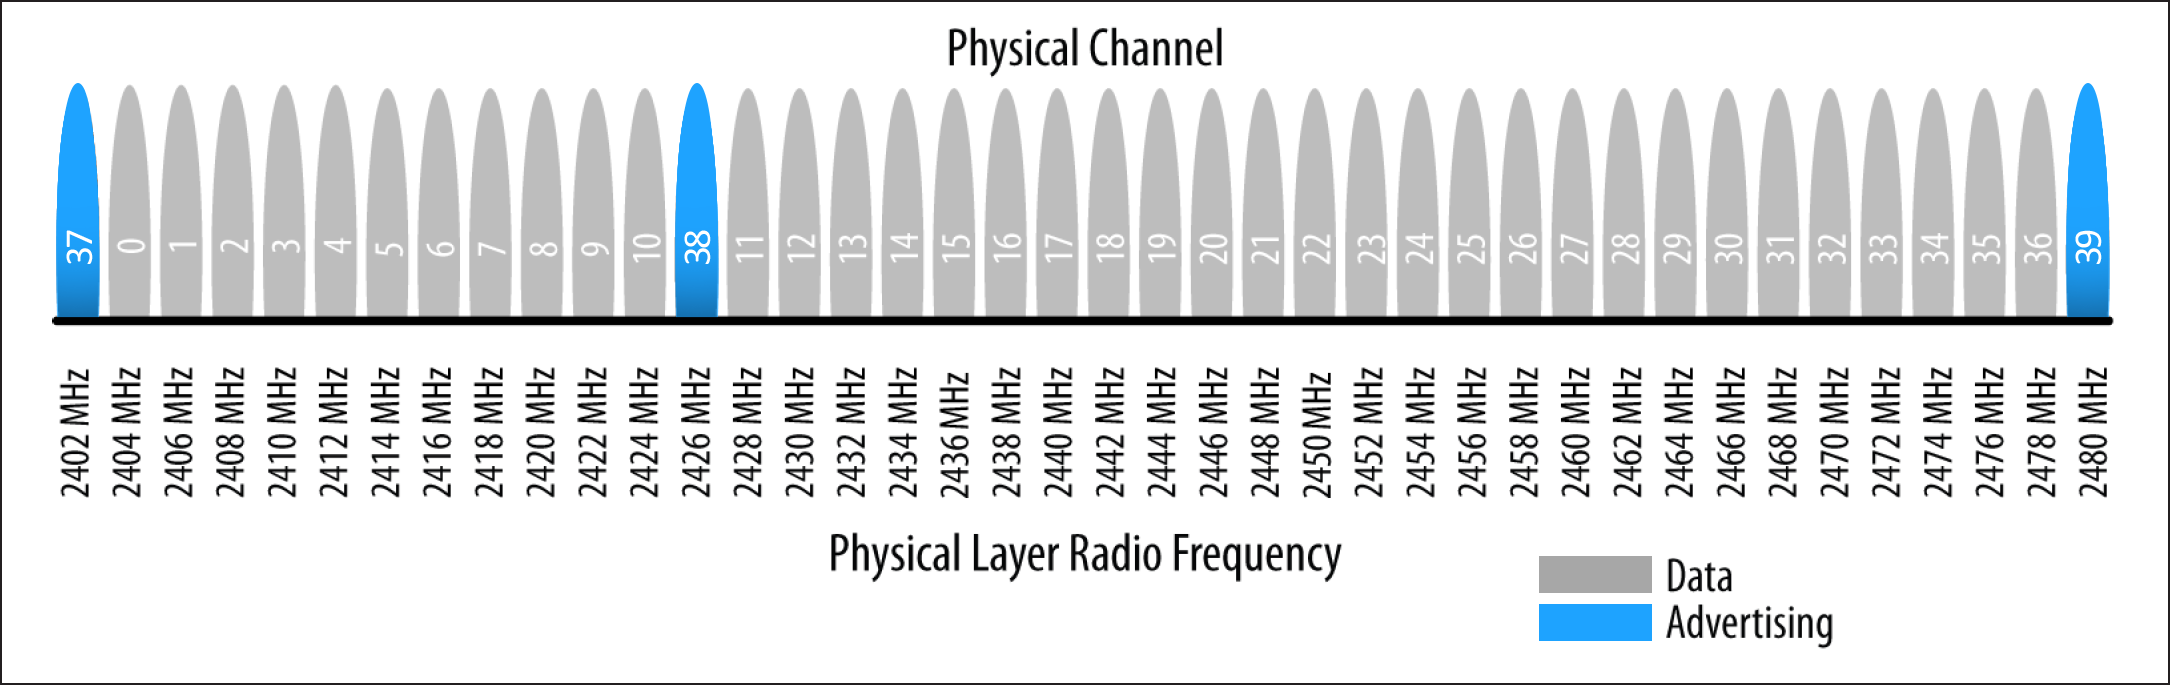
\includegraphics[width = \textwidth]{images/Physical Channel BLE.png}
    \caption{Frequency Channel}
    \label{fig:frequency_channel}
\end{figure}

\noindent Lo standard adotta la tecnica \textit{Frequency Hopping Spread Spectrum} (FHSS), che consente a due dispositivi di cambiare repentinamente frequenza rispettando uno schema apparentemente casuale ma in realtà definito a priori. \\
Il prossimo canale da adottare per un determinato intervallo di tempo viene scelto attraverso la seguente funzione: $ c'=(c+h) \bmod{37}$, in cui $c$ indica il canale attuale, $h$ indica il salto da eseguire e $c'$ denota il prossimo canale per proseguire la comunicazione. L'operazione $\bmod{37}$ consente di muoversi solo nel range dei canali Data. Il valore di $h$, che determina il pattern per la comunicazione, è comunicato dal master nel momento in cui viene stabilita una nuova connessione, all'interno del \textit{connection request packet}.\\
La tecnica FHSS cerca, tra l'altro, di minimizzare gli effetti delle potenziali interferenze radio presenti nell'ambiente circostante (altri dispositivi che usano la banda 2.4 GHz), andando a selezionare uno dei 37 canali disponibili per un determinato intervallo di tempo.\\

% https://www.electronics-notes.com/articles/connectivity/bluetooth/radio-interface-modulation-channels.php
\noindent La tecnica di modulazione usata in BLE per codificare l'informazione digitale in un segnale analogico corrisponde alla Gaussian Frequency Shift Keying (GFSK).
Tale tecnica prevede la rappresentazione dell'informazione digitale e quindi il bit 1 e bit 0, adoperando due frequenze distinte, rispettivamente una deviazione di frequenza positiva e una negativa rispetto alla portante principale. Il segnale modulato viene successivamente filtrato attraverso una curva Gaussiana per garantire che le bande laterali non eccedano troppo rispetto alla portante principale e per rendere più fluide le transizioni. Così facendo si ottiene un'ampiezza di banda di 1 MHz.\\
%Con le versioni successive, per garantire delle velocità di trasmissione maggiori sono state introdotte delle tecniche di Phase Shift Keying (PSK) che prevedono una modifica nella fase del segnale per differenziare i due valori binari. Nello specifico le due tecniche adottate sotto il nome di Enhanced Data Rate (EDR) a partire da Bluetooth2 sono la $\pi/4$ DQPSK e 8DPSK. Si passa da una tecnica all'altra in base al rumore presente nel canale, se le condizioni sono ottime si adopera la 8DPSK consentendo di raggiungere velocità di trasmissioni massime di 3 Mbps, altrimenti si adopera la $\pi/4$ DQPSK che consente un massimo di 2 Mbps. La tecnica di trasmissione dati avanzata, EDR, è implementata come funzionalità aggiuntiva in modo che i dispositivi risultano essere compatibili con le versioni precedenti.\\

\noindent Le potenze del trasmettitore Bluetooth sono piuttosto basse, sebbene ci siano quattro diverse classi energetiche (+20, +10, +4 e 0 dBm) che dipendono dall'uso previsto e dalla distanza di copertura richiesta. Il controllo della potenza è consigliabile al fine di conservare la carica della batteria o ridurre le interferenze con le altre apparecchiature. Il livello di potenza appropriato può essere definito in base al RSSI. La Receiver Sensitivity, ovvero il livello di potenza più basso con la quale è in grado di \textit{rilevare} un segnale RF e \textit{demodulare} i dati contenuti in esso, per i dispositivi che adottano la tecnologia BLE corrisponde a -70 dBm.

\subsubsection{Link Layer (LL)}
% https://medium.com/@pcng/ble-protocol-stack-controller-2d2d5371deec
Il livello di collegamento si interfaccia direttamente con il livello fisico e fornisce un livello di astrazione e il modo per interagire con la radio. Solitamente implementato come una combinazione di hardware e software custom.\\
La parte hardware definisce alcune funzionalità automatizzate, tra cui: Preamble, Indirizzo d'accesso, individuazione del protocollo adoperato, la generazione e verifica del CRC, la generazione del pattern casuale ($h$) e la cifratura attraverso l'algoritmo AES.
La parte software del Link Layer riguarda lo stato dei collegamenti della radio, ovvero il modo in cui il dispositivo si collega ad altri dispositivi. \\
Un dispositivo BLE può agire come master o come slave. Il dispositivo che avvia la connessione sarà il master e i dispositivi che tramite messaggi di Advertisement comunicano la propria presenza e accettano le connessioni, saranno gli slave. 
Solitamente il ruolo del master è rappresentato da dispositivi con più risorse, come smartphone o tablet, mentre ai dispositivi con vincoli di memoria e a basso costo, come microcontrollori o sensori, è riservato il ruolo dello slave.\\

\noindent Il livello di collegamento consente di definire i seguenti ruoli:
\begin{itemize}
    \item \textit{Advertiser}: dispositivo che invia pacchetti Advertising.
    \item \textit{Scanner}: dispositivo che esegue scansioni per individuare la presenza di altri dispositivi nel suo raggio di comunicazione, individuabili tramite la ricezione di pacchetti Advertising.
    \item \textit{Master}: dispositivo che inizializza la connessione. \MakeUppercase{è} responsabile della gestione della connessione, dell'impostazione dei parametri da utilizzare, compresi i timing dei vari eventi, all'interno di una connessione.
    
    \item \textit{Slave}: dispositivo che accetta una richiesta di connessione e si sincronizza con il clock del master.
\end{itemize}

\noindent Quando un dispositivo emette messaggi Advertising attraverso i canali definiti per l'appunto Advertising, consente agli altri device, che sono in una fase di scansione (Scanner), di individuarlo e avere la possibilità di connettersi. Nel momento in cui un Advertiser viene individuato, lo Scanner può decidere di inviare una richiesta di connessione, nella quale è incluso il valore $h$ per definire lo schema di salto di frequenza, per i due dispositivi, durante la connessione. Dopo che l'Advertiser accetta, entrambi passano allo stato \textit{Connection}, assumendo per l'Advertiser il ruolo di Slave e per lo Scanner il ruolo di Master. 
\MakeUppercase{è} possibile definire una \textit{connection} come una sequenza di scambi di dati tra slave e master in momenti prestabiliti. Lo scambio di informazioni, all'interno di una connessione avviene adoperando i canali Data e tramite pacchetti Data (con 27 byte di payload), i quali consentono il trasporto di informazioni utente in entrambe le direzioni.\\
Nello specifico, gli stati in cui si possono trovare i dispositivi BLE sono i seguenti:

\begin{itemize}
    \item \textit{Standby}: lo stato in cui il dispositivo non trasmette e non riceve informazioni. In questo stato è possibile accedere da qualsiasi altro stato.
    
    \item \textit{Advertising}: lo stato in cui il dispositivo invia pacchetti di Advertising individuabili da altri device presenti nell'ambiente circostante. Il dispositivo nello stato di Advertising è conosciuto come Advertiser.
    
    \item \textit{Scanning}: lo stato in cui il dispositivo scansiona l'area circostante in cerca di pacchetti Advertising inviati dagli Advertiser. Il dispositivo nello stato di Scanning è conosciuto come Scanner.
    
    \item \textit{Initiating}: lo stato assunto dal dispositivo che ha ricevuto dei pacchetti Advertising da uno specifico dispositivo e decide di stabilire una connessione con esso.
    
    \item \textit{Connection}: lo stato in cui il dispositivo ha stabilito una connessione con un altro device e regolarmente si scambiano informazioni.
\end{itemize}

\begin{figure}[!ht]
    \centering
    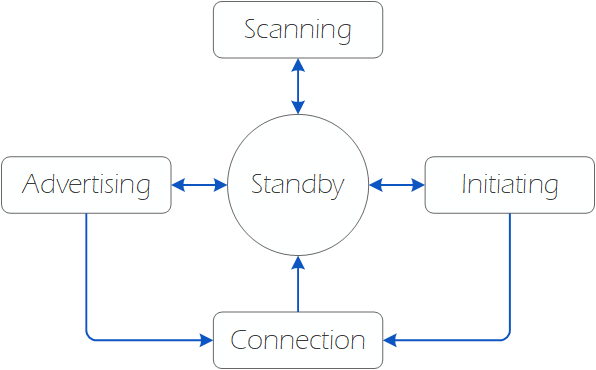
\includegraphics[width = \textwidth]{images/Link layer states.png}
    \caption{Stati Link Layer}
    \label{fig:link_layer_states}
\end{figure}

\noindent Dallo stato Standby è possibile accedere a qualsiasi stato ad eccezioni di Connection, accessibile solo dallo stato Initiating e Advertising.

\paragraph{Device Address}
I dispositivi Bluetooth sono identificabili attraverso un indirizzo di 48 bit (6 byte), \textit{Bluetooth Device Address}, che può essere un \textit{Public device address} o un \textit{Random device address}. 
L'indirizzo \textit{Public} è assegnato al dispositivo al momento della fabbricazione e non cambierà mai per tutta la vita del dispositivo, ed è registrato presso l'autorità IEEE così come avviene per l'indirizzo MAC per i device Wi-Fi o Ethernet. 
L'indirizzo \textit{Random} può essere programmato sul dispositivo o generato dinamicamente in fase di esecuzione. Quest'ultimo è più popolare poiché non richiede la registrazione presso l'ente IEEE.\\
Per quanto riguarda l'indirizzo Random possiamo avere due sottotipi: Static e Private Address.

\begin{itemize}
    \item \textit{Static Address}: in genere sono utilizzati come sostituti degli indirizzi Public. Esso è semplicemente un indirizzo casuale che può essere generato ogni volta che il dispositivo si avvia o definito a priori in modo che rimane invariato ad ogni accensione. Non può essere modificato finché il dispositivo è in esecuzione.
    \item \textit{Private Address}: generati a partire da una Identity Resolving Key (IRK) e da un numero casuale di 24 bit. A differenza dei precedenti, possono essere cambiati spesso, anche mentre il dispositivo è in funzione. Il loro utilizzo è legato alle questioni di privacy, ad esempio si può cambiare l'indirizzo per evitare che il dispositivo venga identificato e rintracciato da un device sconosciuto. Il processo di identificazione può avvenire solo se in possesso della IRK distribuita dal device durante la fase 3 mostrata nel grafico \ref{fig:phasis_pairing_bonding}.
\end{itemize}

\paragraph{Advertising e Scanning}
BLE ha solo un formato per i pacchetti, però possiede due tipologie di pacchetti: Advertising e Data. 
I pacchetti Advertising possono avere un payload di dimensioni fino ad un massimo 31 bytes. Essi sono inviati in broadcast dal dispositivo Advertiser senza essere a conoscenza della presenza di un eventuale device Scanner. L'invio avviene con un intervallo prefissato compreso tra 20ms e 10.24ms, con incrementi di 625 $\mu s$. Più corto è l'intervallo e più alta è la frequenza con cui i pacchetti sono inviati in broadcast, aumentando così la probabilità di essere intercettati dai dispositivi in ascolto, ma compromettendo la durata della batteria, difatti l'uso di una frequenza più alta comporta un maggior consumo di energia. Solitamente si tende a privilegiare un intervallo alquanto lungo che fornisce equilibrio tra connettività rapida e consumo energetico ridotto.\\
Il processo di Advertising predispone al massimo tre canali e poiché l'advertiser e lo scanner non risultano sincronizzati, un pacchetto Advertising verrà ricevuto sono quando i rispettivi intervalli di invio e ascolto si sovrapporranno. I parametri che consentono di gestire tale situazione sono: \textit{Scan Type} che può essere passivo o attivo, \textit{Scan Window} indica per quanto tempo può essere in ascolto sui canali di Advertising e \textit{Scan Interval} indica quanto spesso eseguire il processo di ascolto. Difatti lo Scanner sarà in ascolto sui tre canali di Advertising per l'intera durata della Scan window ed ogni Scan Interval.\\ 
% Immagine Passive e active scanning pagina 35
In merito alla scansione dei pacchetti Advertising sono definite due modalità: \textit{Passive scanning} e \textit{Active scanning}.
Durante una procedura passiva, lo scanner semplicemente si mette in ascolto di eventuali messaggi, e l'Advertiser non sarà mai a conoscenza se uno o più pacchetti saranno effettivamente ricevuti dai dispositivi circostanti.
Con la procedura attiva, lo scanner inoltra una Scan Request dopo aver ricevuto un pacchetto Advertising. In tal modo, l'Advertiser riceverà la richiesta e sarà per prima cosa a conoscenza dell'avvenuta ricezione, dopodiché procederà a rispondere attraverso una Scan Response. L'uso di Scan Request e Response consente all'Advertiser di inviare informazioni aggiuntive che non rientrerebbero nel normale pacchetto Advertising. \\
I pacchetti Advertiser sono utilizzati dai livelli superiori, più specificamente, dal GAP per differenziare le modalità operative e definire le procedure.

\paragraph{Connections}
Per stabilire una connessione tra due dispositivi Bluetooth, per prima cosa si deve avere un dispositivo con il ruolo di Advertiser ed uno con il ruolo di Scanner. Detto ciò, il dispositivo nello stato di Advertising inizia ad inviare pacchetti per testimoniare la sua presenza e il dispositivo nello stato di Scanning , nel mentre, deve scansionare l'intera area al fine di acquisire i pacchetti inviati dall'altro device. I pacchetti riscontrati, verranno filtrati attraverso il Bluetooth Address o in base alla tipologia. \\
Quando, a seguito dell'analisi dei pacchetti intercettati, viene riscontrata la presenza di un potenziale slave, il nodo Central procederà con l'invio di una richiesta di connessione (Connection Request packet). Il nodo periferico è sempre in ascolto per un breve intervallo di tempo sugli stessi canali utilizzati per inviare pacchetti Advertising. Ciò gli consente di ricevere il pacchetto Connection Request il quale innescherà un processo di connessione tra i due dispositivi, il che comporterà l'invio di una risposta da parte dello slave, sempre se desidera procedere in tale direzione.\\
Solo nel momento in cui verrà ricevuto quest'ultimo pacchetto la connessione si può considerare stabilita, altrimenti essa risulta solo creata. Solo dopo aver instaurato la connessione è possibile definire il nodo Central come Master e il nodo Peripheral come Slave.\\

\begin{figure}[!ht]
    \centering
    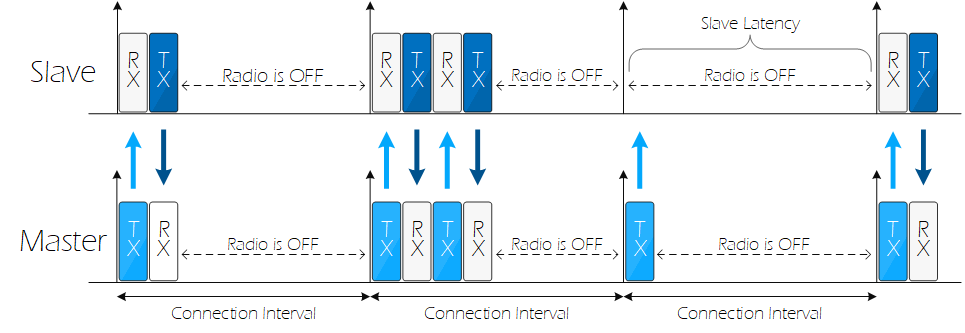
\includegraphics[width = \textwidth]{images/Connection events.png}
    \caption{Connection events}
    \label{fig:connection_events}
\end{figure}

\noindent La connessione è semplicemente una sequenza di scambio di dati tra master e slave, in modo alternato e in istanti prestabiliti. L'invio alternato dei pacchetti dati costituisce il \textit{Connection Event}. Tale evento prevede sempre la presenza di almeno un pacchetto inviato dal master a cui fa seguito la risposta da parte dello slave. Se il master non riceverà risposta da parte dello slave chiuderà il connection event e riprenderà l'invio al successivo connection event. Il tempo trascorso tra l'inizio di due connection event successivi è chiamato \textit{Connection Interval}. Questo asso temporale corrisponde ad un valore compreso tra 7.5 ms (alto throughput) e 4 s (basso throughput) con soglie di 1.25 ms. Altri parametri impostati prima di stabile la connessione riguardano lo \textit{Slave Latency} e \textit{Connection Supervision Timeout}.\\
Il parametro slave latency consente al dispositivo peripheral di scegliere un numero consecutivo di connection event da saltare senza compromettere la connessione. Questo consente al dispositivo di restare spento per un lungo periodo di tempo, potenzialmente riducendo i consumi energetici.\\
Il parametro connection supervision timeout definisce il tempo massimo tra la ricezione di due pacchetti dati prima che la connessione venga considerata persa. L'intervallo è compreso tra 100 ms e 32 s con soglie di 10 ms.\\

\noindent Un nodo BLE prima di accedere al contenuto di un pacchetto ricevuto, può attuare un meccanismo di filtering il quale consente di scartare quei pacchetti a cui non è interessato. Una \textit{White List} è semplicemente una lista di Bluetooth device address popolata dall'host e memorizzata ed utilizzata dal controller. Tale lista può essere utilizzata per gli stati di Advertising, Scanning e Initiating.


\subsubsection{Host Controller Interface (HCI)}
Come introdotto in precedenza, la specifica Bluetooth definisce l'HCI come uno standard per consentire l'interazione tra Host e Controller all'interno di uno stack BLE. Questi livelli possono essere implementati come chipset differenti o possono coesistere nel medesimo chipset. Nel caso in cui i due livelli sono in due chipset differenti, il livello HCI sarà implementato su un'interfaccia di comunicazione fisica, mentre nel caso in cui si trovano nel medesimo chipset, allora HCI sarà un'interfaccia logica.\\
Il ruolo di HCI layer prevede la trasmissione dei comandi dal host verso il controller e viceversa.

\subsubsection{Logical Link Control and Adaptation Protocol (L2CAP)}
Il livello L2CAP fornisce due funzionalità importanti per lo standard BLE. Innanzitutto, consente di incapsulare tutti i protocolli degli strati superiori all'interno di un pacchetto standard BLE. Inoltre, esegue il processo di frammentazione nel momento in cui, dai livelli superiori, giunge un pacchetto le cui dimensioni risultano maggiori dello standard BLE (Payload LL layer 27 byte e 4 byte header L2CAP); mentre, nel caso in cui giunge un pacchetto frammentato, attende la ricezione di tutti i frammenti prima di procedere con la creazione del pacchetto originale e l'invio all'entità appropriata di livello superiore. La frammentazione è poco adoperata in primo luogo perché richiede un dispendio piuttosto elevato di energia e in più perché gli standard utilizzati ai livelli superiori consentono di fornire unità dati che si adattano alla dimensione massima del payload L2CAP, di 23 byte in BLE. \\
Per BLE, il protocollo L2CAP è responsabile di due protocolli principali: Attribute Protocol (ATT) e Security Manager Protocol (SMP). Il protocollo ATT costituisce la base per lo scambio di informazioni per applicazioni BLE, mentre SMP fornisce un framework per generare e distribuire le chiavi di sicurezza tra i nodi.

\subsubsection{Attribute Protocol (ATT)}
L'Attribute Protocol è un protocollo che definisce la comunicazione tra due dispositivi con il ruolo di client e server per accedere agli \textit{attributi} forniti dal server. Più specificamente, definisce come un server espone i propri dati ad un client e come tali dati risultano strutturati.
Il server è quel dispositivo che accetta richieste eseguite da un dispositivo ed invia risposte, notifiche e indicazioni in merito ai propri attributi. % Esempio di Server: Termometro quando espone la temperatura dell'ambiente circostante
Il client invece, è quel dispositivo che interagisce con il server con lo scopo di entrare a conoscenza dei dati esposti dal server e all'occorrenza controllare il comportamento del server. Il client non è a conoscenza degli attributi forniti dal server, quindi prima deve informarsi sulla presenza e sulla natura di tali attributi attraverso la procedura di service discovery, dopodiché può dare il via alle operazioni di reading e writing degli attributi individuati.\\
I dati messi a disposizione dal server sono organizzati secondo una struttura dati predefinita e generica che prende il nome di \textit{attributo}, manipolati e acceduti attraverso il protocollo GATT.\\
A ciascuno attributo è assegnato un identificativo univoco di 128 bit (16 byte),\textit{Universally Unique Identifier} o UUID, che ne specifica il tipo e la natura dei dati, oltre a consentire l'accesso alla risorsa. Per questioni di efficienza, la specifica BLE definisce un formato addizionale di 16 bit. Il formato ridotto (16 bit) può essere adottato solo per quegli attributi definiti nella specifica Bluetooth (definiti come standard da parte di Bluetooth SIG). \\
Nel caso in cui si abbia la necessità di una specifica non definita dallo standard SIG, è possibile implementarla e assegnargli un UUID specifico di 128 bit, denominata come \textit{vendor-specific UUID}.
%% Attribute handle
L'\textit{attribute handle} è un identificatore di 16 bit, presente in ogni attributo, che permette ad una specifica risorsa di essere reperibile dal client, e garantisce l'identificazione univoca per tutta la durata di una connessione.\\
%% Type e Value
Il campo \textit{type} incluso all'interno di un attributo è legato al rispettivo UUID e determina il tipo di dato presente nel campo \textit{value} e i meccanismi individuabili nella fase di discovery per poter accedere a tale attributo.\\
%% Permission
I \textit{permessi} sono metadati presenti in ogni attributo e specificano quale operazione ATT può essere eseguita e quali sono i requisiti di sicurezza per potervi accedere. Possono essere distinti in: Access Permission, Encryption e Authorization.
\begin{itemize}
    \item \textit{Access Permission}: determina se il client ha il permesso in lettura o in scrittura (o entrambe) al valore di un attributo.\\
    \textit{None} indica che il client non ha i permessi né per la lettura né per la scrittura.
    \textit{Readable} indica che l'attributo può essere accessibile solo in lettura.
    \textit{Writable} indica che il client ha il permesso in scrittura per l'attributo.
    Se l'attributo presenta entrambi i permessi, \textit{Readable} e \textit{Writable}, allora il client può accedere sia in lettura sia in scrittura.
    
    \item \textit{Encryption}: determina il livello di sicurezza richiesto per far sì che il client possa accedere ad un determinato attributo.
    \textit{No encryption required} indica che l'attributo è accessibile senza nessun livello di sicurezza, le informazioni sono accessibile senza avere una comunicazione cifrata.
    \textit{Unauthenticated encryption required} prevede l'utilizzo di una connessione cifrata per accedere all'attributo, ma non necessita che le chiavi di cifratura siano autenticate.
    \textit{Authenticated encryption required} garantisce il livello di sicurezza più alto, vale a dire che per accedere all'attributo la connessione deve essere crittografata con una chiave autenticata.
    
    \item \textit{Authorization}: determina se l'accesso all'attributo prevede l'autorizzazione da parte dell'utente. Le alternative in questa circostanza sono \textit{No authorization required} o \textit{Authorization required}.
\end{itemize}
\noindent Il \textit{permesso}, in realtà, non viene definito o individuato attraverso il protocollo ATT, bensì attraverso il protocollo GATT o il livello Applicativo.\\

\noindent Il protocollo ATT opera in termini di attributi e tramite essi è in grado di fornire una serie di Protocol Data Unit (PDU o packet) che consentono ad un client ad accedere agli attributi su un server.

\subsubsection{Security Manager (SM)}
La sicurezza è una delle maggiori preoccupazioni espresse nel contesto dei sistemi IoT. Tra le problematiche più comuni in merito alla sicurezza per sviluppatori e produttori di dispositivi, si hanno:
\begin{itemize}
    \item \textit{Autenticazione}: essere sicuro che l'altra parte sia davvero chi afferma di essere.
    \item \textit{Integrità}: assicura che i dati non risultano corrotti e manomessi da un utente o dispositivo non autorizzato a trattarli.
    \item \textit{Riservatezza}: essere sicuri che i dati non siano leggibili da dispositivi o utenti non autorizzati.
    \item \textit{Privacy}: indica quanto è privata una comunicazione e se una terza parte è in grado di tracciare il nostro dispositivo, soprattutto dal suo identificativo.
\end{itemize}
In merito alla sicurezza ed ai concetti appena espressi, purtroppo ci sono differenti tipi di attacchi che possono essere messi in atto da un soggetto malintenzionato. Alcuni di essi riguardano:
\begin{itemize}
    \item \textit{Intercettazione Passiva}: si verifica nel momento in cui un malintenzionato si posiziona tra i due dispositivi, ascoltando la comunicazione e riuscendo a comprendere il suo contenuto. Solitamente ottenendo l'accesso alla chiave di cifratura nel momento in cui i dati risultano cifrati.
    \item \textit{Intercettazione Attiva}: attacco conosciuto anche con il nome di \textit{Man-In-The-Middle} (MITM). 
    Tipologia di attacco informatico in cui un soggetto malintenzionato cerca di intercettare e alterare la comunicazione tra due entità che credono di comunicare direttamente tra loro. Più nello specifico, l’attaccante si colloca letteralmente nel mezzo tra le due entità, in questo modo riesce non solo a intercettare i messaggi inviati e ricevuti, ma può anche modificarli o fingersi una delle due parti. Il tutto, senza che le due entità riescano a comprendere ciò che sta succedendo.
    \item \textit{Monitoraggio della Privacy e dell'identità}: in questa tipologia di attacco, il dispositivo è tracciato tramite l'indirizzo Bluetooth con la possibilità di individuare la sua posizione e correlandola con il suo comportamento.
\end{itemize}

\noindent Security Manager è sia un protocollo sia una serie di algoritmi di sicurezza progettati per fornire la capacità di generare e scambiare chiavi di sicurezza al fine di garantire una comunicazione attraverso un collegamento criptato. Comprende cinque funzioni:
\begin{itemize}
    \item \textit{Pairing}: procedura mediante la quale viene generata una chiave segreta, condivisa tra i due dispositivi, al fine di costituire un collegamento crittografato e sicuro. Tale chiave risulta essere temporanea, quindi non potrà essere riutilizzata per le connessioni successive.
    
    \item \textit{Bonding}: il processo di creazione e archiviazione della chiave segreta eseguito da entrambi i dispositivi, che consentirà loro di impostare rapidamente un collegamento sicuro anche per le connessioni successive.
    
    \item \textit{Autenticazione}: il processo che consente di verificare che entrambi i dispositivi condividono la stessa chiave segreta.
    
    \item \textit{Crittografia}: il processo prevede di crittografare i dati scambiati tra due dispositivi. In BLE tale processo avviene utilizzando lo standard di cifratura AES a 128 bit, algoritmo di cifratura a chiave simmetrica (significa che la stessa chiave è usata sia per cifrare che per decifrate i dati su entrambi i lati).
    
    \item \textit{Integrità dei messaggi}: il processo che consente di controfirmare i dati e verificare la validità della firma sull'altro dispositivo.
\end{itemize}
Il \textit{Pairing} consente di creare un collegamento sicuro che durerà solo per la durata della connessione, mentre il \textit{Bonding} crea effettivamente un'associazione permanente sotto forma di chiavi di sicurezza condivise utilizzabili per le connessioni future, finché i due nodi non decidono di eliminarle. La fase di Bonding consente ai due dispositivi, nel momento in cui dovranno creare nuovamente un canale di comunicazione sicuro, di evitare la fase di Pairing.\\

\noindent In BLE i diversi problemi menzionati all'inizio del capitolo sono affrontati tramite le funzioni appena descritte, ovvero: la \textit{riservatezza} viene garantita attraverso il processo di crittografia dei dati; l'\textit{autenticazione} tramite le funzioni di pairing e bonding; la \textit{privacy} è garantita adottando gli indirizzi privati; l'\textit{integrità dei dati} viene assicurata tramite il meccanismo di firma digitale.

\begin{figure}[!ht]
    \centering
    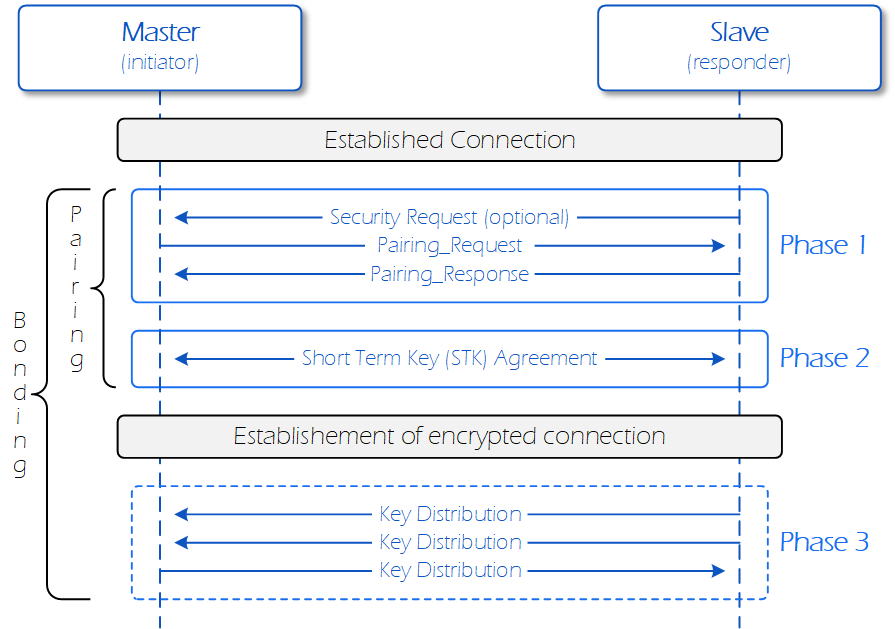
\includegraphics[width = \textwidth]{images/Pairing and Bonding.png}
    \caption{Fasi del processo di sicurezza in BLE}
    \label{fig:phasis_pairing_bonding}
\end{figure}

\noindent Il processo che consente di rendere il collegamento tra due dispositivi sicuro (mostrato in figura \ref{fig:phasis_pairing_bonding}), prevede innanzitutto uno scambio di informazioni per generare una chiave di sicurezza temporanea (fase 1) e, opzionalmente questa fase può essere avviata da una richiesta eseguita da parte dello slave per l'avvio di una procedura di sicurezza. Lo scambio di informazioni avviene attraverso lo scambio di messaggi tra master e slave, ed è il master ad avviare il processo inviando il messaggio \textit{Pairing Request} a cui lo slave risponde con il messaggio \textit{Pairing Response}, in questo caso il master è denominato \textit{initiator} mentre lo slave \textit{responder}. Le informazioni scambiate in questa fase determinano il metodo da utilizzare per la procedura di Pairing, ovvero la fase 2.\\
Dopo di che, (fase 2) entrambi i dispositivi generano in modo indipendente una chiave cifrata temporanea (\textit{Short Term Key} o STK) e la usano per crittografare la connessione. 
Una volta che la connessione risulta essere cifrata e solo se si utilizza la procedura di \textit{Bonding} (fase 3), le chiavi permanenti possono essere distribuite per la memorizzazione e il riutilizzo in un secondo momento. 

\subsubsection{Generic Attribute Profile (GATT)}
Generic Attribute Profile è implementato al di sopra di Attribute Protocol (ATT), aggiunge una gerarchia e un modello di astrazione ai dati. Adoperato solo dopo avere instaurato una connessione tra due dispositivi, risulta l'elemento cardine all'interno di una comunicazione BLE. Il protocollo GATT definisce la struttura e le regole attraverso cui i dati, esposti dal server, devono essere scambiati tra due applicazioni. A tal proposito sono introdotti concetti come \textit{Services} e \textit{Characteristics} per specificare la struttura dei dati e le procedure per interfacciarsi con gli attributi definiti (come service discovery, la lettura e  la scrittura delle caratteristiche, le notifiche, etc.).\\
Il ruolo di client e server non è definito a priori, esso è determinato in base alla circostanza ($request \leftrightarrow{response}$, $indication \leftrightarrow{confirmation}$ e $notification$). Vale a dire che un dispositivo, all'interno di una connessione, può agire sia come server mettendo a disposizione i propri dati per i client, sia come client leggendo dati messi a disposizione da altri server.

\paragraph{Profiles, Services e Characteristics}
Il protocollo GATT prevede di raggruppare gli attributi correlati tra loro, al fine di definire una funzionalità specifica del server, attraverso una struttura dati gerarchica denominata \textit{service}.\\

\noindent Un service è costituito sempre da una \textit{service declaration}, posta sempre come primo attributo, e seguita da zero o più \textit{characteristics}. A seguito della dichiarazione possono essere aggiunti zero o più attributi \textit{include definitions}, i quali consentono di richiamare altri service al fine di estendere le funzionalità. Il campo conterrà tutti i dettagli richiesti affinché il client possa far riferimento al service aggiunto.\\
I service possono essere divisi in primario e secondario. Il primary rappresenta le funzionalità standard fornite dal server GATT, mentre il secondary definisce delle funzionalità aggiuntive e può essere incluso solo al seguito di un primary.

\begin{figure}[!ht]
    \centering
    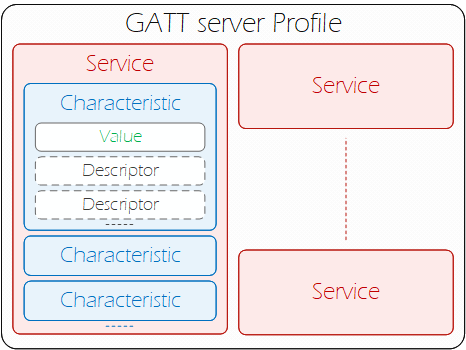
\includegraphics[width =\textwidth]{images/Services GATT.png}
    \caption{Profile, Services e Characteristics}
    \label{fig:profile_GATT}
\end{figure}

\noindent La caratteristica, sempre compresa in un service, rappresenta l'informazione che il server vuole esporre ai client. Comprende sempre almeno due attributi: \textit{characteristic declaration} che fornisce informazioni in merito ai dati che detiene e \textit{characteristic value} contenente i dati effettivi sui quali il client può accedere sia in lettura che in scrittura. Quest'ultimo campo può essere seguito da zero o più \textit{descriptors} in grado di espandere ulteriormente i metadati contenuti nella dichiarazione.\\
L'attributo \textit{declaration}, ha l'autorizzazione ad essere acceduto solo in lettura ed è ripartito in diversi campi, tra cui il campo \textit{Properties} contenente le operazioni e le procedure eseguibili dal client sulla specifica caratteristica.\\
% Ad esempio, il \textit{battery service} definito da SIG contiene una caratteristica chiamata \textit{battery level}. 

\noindent I \textit{Profiles} sono molto più ampi nella definizione rispetto ai service e il loro compito è di definire il comportamento, sia del client sia del server, quando si tratta di servizi, caratteristiche e persino connessioni e requisiti di sicurezza. I service e le rispettive specifiche invece, si occupano dell'implementazione solo lato server. Così come per i service, anche per i profile ci sono standard definiti da Bluetooth SIG e generalmente comprendono la definizione dei ruoli e relazioni tra server e client, i requisiti per i service e come utilizzarli assieme alle caratteristiche richieste, le considerazioni in ambito di sicurezza e persino i dettagli che definiscono i criteri e i requisiti necessari per garantire una connessione.

\subsubsection{Generic Access Profile (GAP)}
Il protocollo Generic Access Profile definisce i ruoli, i modi e le procedure al fine di assicurare l'interoperabilità e lo scambio di informazioni tra dispositivi realizzati da fornitori diversi, oltre a definire un insieme di regole e concetti per regolare e standardizzare le operazioni svolte nei livelli sottostanti.
Nello specifico determina come i dispositivi devono eseguire le procedure di controllo come la discovery dei dispositivi e dei services, la gestione dell'instaurazione della connessione, l'instaurazione in un collegamento sicuro, ed eseguire molte altre operazioni fondamentali dello standard BLE.\\

\noindent Tale protocollo definisce i seguenti aspetti legati all'interazione tra dispositivi.
\paragraph{Ruoli}
Ogni dispositivo può operare in uno o più ruoli contemporaneamente e ognuno di essi impone restrizioni e determinati requisiti in merito al comportamento. Alcune combinazioni consentono ai dispositivi di comunicare tra loro e il protocollo GAP stabilisce le interazioni tra tali ruoli. I quali possono essere:
\begin{itemize}
    \item \textit{Broadcaster}: invia periodicamente pacchetti Advertising contenenti i dati. Ottimizzato per applicazioni che necessitano solo distribuire i dati regolarmente. Un ottimo esempio potrebbe essere un termometro in grado di trasmettere le letture a tutti i dispositivi interessati. Il Broadcaster invia dati all'interno di pacchetti Advertising e non attraverso pacchetti Data, utilizzabili solo a seguito di una connessione. In tal modo, i dati sono accessibili a qualsiasi dispositivo in ascolto. Broadcaster si basa sul ruolo Advertiser del Link Layer.
    
    \item \textit{Observer}: nodo improntato all'ascolto dei messaggi Advertising inviati dai nodi circostanti. Ottimizzato per le applicazioni che desiderano solo raccogliere informazioni provenienti dai nodi Broadcaster. Un esempio potrebbe essere un dispositivo dotato di display tramite il quale mostra i dati delle temperature ricevute da sensori di temperatura broadcaster.  Non ha la capacità di avviare una connessione con l'Advertiser e si basa sul ruolo di Scanner del Link Layer.
    
    \item \textit{Central}: un dispositivo in grado di stabilire connessioni multiple con i nodi e corrisponde al ruolo di Master per il Link Layer. Il protocollo BLE è \textit{asimmetrico}, il che significa che i requisiti del master sono maggiori rispetto a quelli dello slave e, a tal proposito il ruolo di Central è svolto solitamente da dispositivi in possesso di CPU performanti e con ottime capacità di memoria, come lo sono gli smartphone o tablet. Proprio la presenza di tali requisiti rende possibile mantenere connessioni tra più dispositivi. 
    
    \item \textit{Peripheral}: dispositivo che si preoccupa di inviare pacchetti Advertising per consentire ai nodi Central di individuarlo, e successivamente, stabilire una connessione con esso. Una volta che viene instaurata una connessione con un dispositivo Central, diventa noto anche come Slave in tale connessione, arresta l'invio di pacchetti Advertising. Ottimizzato al fine di minimizzare le risorse necessarie per la sua implementazione, in termini di potenza di elaborazione e memoria.
\end{itemize}

\noindent Confrontando i ruoli definiti attraverso il protocollo GAP e quelli individuabili attraverso il protocollo GATT possiamo affermare che le mansioni di client e di server dipendono esclusivamente dalla direzione in cui fluiscono le transazioni di richiesta e risposta in merito ai dati, mentre i ruoli definiti dal protocollo GAP, sopra descritti, rimangono invariati.\\

\noindent Un tipico esempio di applicazioni basate sul ruolo di Broadcaster sono le tecnologie \textit{Beacon}. I Beacon sono dispositivi aventi il solo scopo di pubblicizzare la propria esistenza e trasmettere dati specifici, mentre non sono in grado di accettare connessioni da altri dispositivi.\\

\noindent Il modo in cui un Broadcaster si differenzia da un nodo Peripheral è attraverso i pacchetti Advertising trasmessi dal dispositivo. Esistono due tipi di pacchetti Advertising: alcuni consentono di accettare le connessioni, mentre altri servono solo per pubblicizzare la propria presenza. Quando un dispositivo Central riceve un pacchetto Advertising è in grado di comprendere il ruolo del dispositivo mittente e quindi se è possibile instaurare una connessione.\\
Il principale vantaggio di restare nello stato di Advertising è che molti dispositivi possono scoprire Advertising Data senza la necessità di instaurare una connessione. Tuttavia, l'aspetto negativo riguarda la mancanza di sicurezza e l'impossibilità di instaurare una comunicazione bidirezionale (dal Central al Broadcaster).

\begin{figure}[!ht]
    \begin{subfigure}{0.5\textwidth}
        \centering
        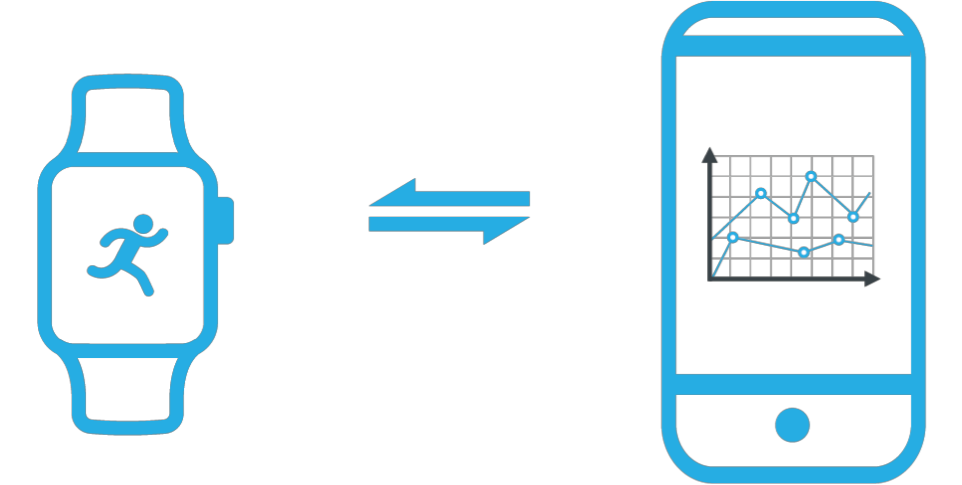
\includegraphics[width=0.85\linewidth]{images/Peripheral - Master.png} 
        \caption{Peripheral - Central}
        \label{fig:subim1}
    \end{subfigure}
    \begin{subfigure}{0.5\textwidth}
        \centering
        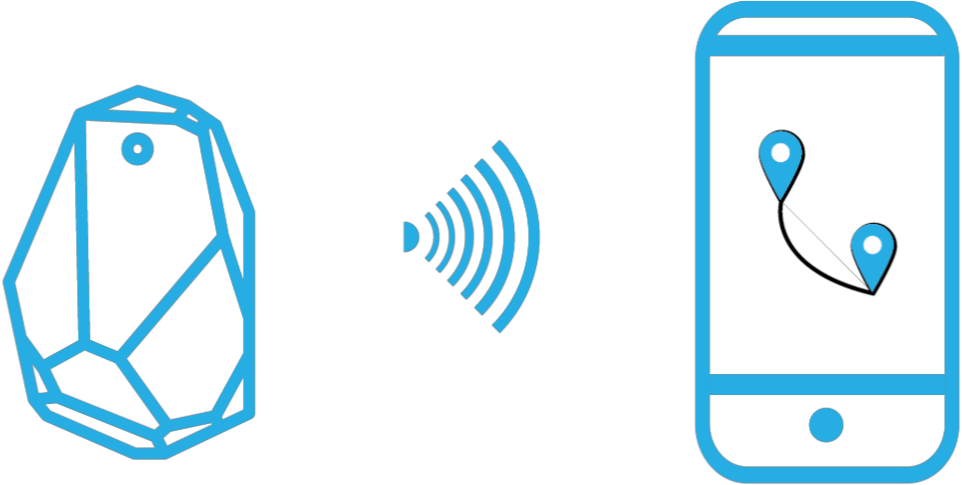
\includegraphics[width=0.85\linewidth]{images/Broadcaster - Observer.png}
        \caption{Broadcaster - Observer}
        \label{fig:subim2}
    \end{subfigure}
    \caption{Ruoli dei dispositivi BLE definiti dal protocollo GAP}
    \label{fig:GAP_roles}
\end{figure}

\noindent Ricapitolando, si può affermare che i ruoli di Broadcaster e Observer necessitano di risorse piuttosto limitate e non garantiscono una comunicazione bidirezionale, poiché rispettivamente provvedono a trasmettere e ricevere informazioni tramite pacchetti Advertising. Gli altri due ruoli, Peripheral e Central, invece necessitano dell'intero stack BLE il che consente loro di supportare una comunicazione bidirezionale. Gran parte delle responsabilità di elaborazione devono essere svolte dal dispositivo centrale consentendo così di ridurre i consumi energetici per i dispositivi periferici e dando loro la possibilità di essere rappresentati attraverso dispositivi sempre più piccoli, con risorse limitate e alimentati a batteria.

\paragraph{Modalità e Procedure}
La modalità è uno stato in cui il dispositivo può passare per un certo periodo di tempo al fine di raggiungere un determinato obiettivo o, più specificamente, consentire ad un nodo ad eseguire una determinata procedura. 
Una procedura è una sequenza di azioni che consentono ad un dispositivo il raggiungimento un determinato obiettivo. Una procedura è solitamente associata ad una modalità su un altro nodo, a tal proposito sono spesso messe in relazione.
Il passaggio da una modalità all'altra può avvenire a seguito di azioni innescate tramite l'interfaccia utente o automaticamente quando richiesto.\\

\noindent La modalità \textit{broadcast} e la procedura \textit{observation} definite da GAP rappresentano l'approccio attraverso il quale i dispositivi possono inviare i dati unidirezionalmente. Un broadcaster invia in broadcast dati senza alcuna conferma o riscontro e non ha nessun modo per verificare se i dati inviati raggiungono effettivamente altri dispositivi, mentre un observer ascolta potenziali broadcaster senza alcuna garanzia di ricevere effettivamente informazioni.\\

\noindent La \textit{discoverability} si riferisce al modo in cui un dispositivo pubblicizza la propria presenza e cosa possono o dovrebbero fare i dispositivi in ascolto con le informazioni ricevute dai dispositivi nelle vicinanze. Ciò non implica necessariamente
l'intenzione di creare una connessione o scambiare i dati. Ci sono diverse modalità in merito alla discoverability che consentono una certa flessibilità ai progettisti di nodi periferici, a seconda della priorità di progettazione come ad esempio durata della batteria piuttosto che tempi di connessione rapidi.\\

\noindent La modalità \textit{connectable} consente di far stabilire una connessione tra un dispositivo central ed uno periferico. A seconda della modalità di creazione di una connessione si riflette sull'uso dei diversi pacchetti Advertising per un dispositivo periferico.

\paragraph{Sicurezza}
Il protocollo GAP in merito alla sicurezza definisce modalità e procedure di sicurezza che specificano il modo in cui i nodi impostano il livello di sicurezza richiesto da un particolare scambio di informazioni e successivamente come viene applicato tale livello di sicurezza. Le funzionalità definite non sono associate ad una particolare modalità o procedura, proprio per questo motivo possono essere utilizzate per aumentare il livello di sicurezza dei dati gestiti da qualsiasi tipo di applicazione.\\

\noindent Gli aspetti di sicurezza per BLE sono basati su due pilastri: il protocollo SM e gli aspetti GAP in merito alla sicurezza.\\
Il protocollo SM implementa gli algoritmi di crittografia e si occupa di tutte quelle funzionalità che consentono lo scambio di dati in modo sicuro tra due dispositivi.\\
GAP definisce una serie di modalità e procedure relative alla sicurezza le quali consentono di instaurare una connessione fidata e in grado di trasportare dati sensibili. Inoltre, GAP espande e specifica ulteriormente l'utilizzo degli strumenti definiti dal protocollo Security Manager al fine di garantire interoperabilità tra dispositivi differenti.

\section{ZigBee}
%%% LIBRO ZIGBEE [1,4,5 ]
ZigBee è uno degli standard più popolari sul mercato, per reti di sensori a basso costo, a bassa velocità trasmissiva, a basso consumo energetico a corto raggio \cite{farahani2011zigbee}. ZigBee è definito come protocollo di comunicazione di alto livello, basato sullo standard IEEE 802.15.4, il quale è stato definito per l'implementazione e la standardizzazione di reti Wireless PAN (Personal Area Network) a bassa velocità di comunicazione.\\

\noindent Le applicazioni che prediligono l'uso della tecnologia ZigBee sono alimentate a batteria, e devono soddisfare le caratteristiche definite dalla tecnologia in uso, come: basso costo, bassa potenza, limitata velocità di trasmissione dati e lunga durata della batteria. Tali applicazioni prediligono un uso molto limitato della radio, difatti il dispositivo spende la maggior parte del suo tempo in modalità risparmio energetico, noto anche come \textit{sleep mode}.
Queste caratteristiche, insieme al funzionamento su uno spettro di frequenze libero, senza licenza, previsto dallo standard IEEE 802.15.4 (che definisce i livelli fisico e di collegamento), facilitano lo sviluppo e l'implementazione della rete e la rendono una delle tecnologie wireless più adatte per le applicazioni di smart grid \cite{yi2010developing}.\\

\noindent Gli studi di tale protocollo sono iniziati a partire dal 1998 da parte della Motorola. In seguito, nel 2002, fu fondata la ZigBee Alliance, un'associazione non profit composta da un centinaio di aziende associate, tra cui Motorola, Philips, Samsung, Mitsubishi, Texas Instruments che operano nel campo dei semiconduttori, tecnologia hardware e software, sistemi di comunicazione e prodotti end-user. Lo sviluppo dello standard ZigBee da parte di tale Associazione è avvenuto per rispondere all'esigenza di realizzare reti stabili caratterizzate da un basso consumo, da un ridotto consumo energetico e di estrema facilità d'uso, anche a costo di un bit rate relativamente basso. Nel 2005, la ZigBee Alliance ha rilasciato la specifica 1.0 nella quale definiva i criteri in merito al livello di rete e di applicazione.

\subsubsection{Aspetti Tecnici}
Le sue regole di funzionamento lo rendono un sistema abbastanza robusto in presenza di rumore, in quanto prima di inviare le informazioni verso il livello fisico queste vengono modulate utilizzando le tecniche DSSS (Direct Sequence Spread Spectrum) e PSSS (Parallel Sequence Spread Spectrum). % 12
ZigBee è in grado di operare sulle bande UHF (868 e 915 MHz) e ISM (2.4 GHz), con velocità di trasmissione dati compresa tra 20 kbps e 250 kbps.\\ % ISM - Industrial, Scientific, Medical frequency bands
Anche questa tecnologia è di prossimità, difatti il raggio d'azione non supera le decine di metri su singola tratta (single-hop), ma è possibile estenderlo andando a creare una rete di dispositivi e sfruttando l'approccio ``multi-hop'', il quale consente di far transitare l'Informazione da un nodo all'altro fino al nodo destinazione, che non trovandosi nel raggio di comunicazione del nodo mittente, non può essere raggiunto direttamente.\\
Come definito dalla specifica 802.15.4, si possono adottare due modalità di comunicazione, \textit{beacon-enabled} e \textit{non-beacon-enabled}. A seconda del modello adottato dai nodi costituenti una rete ZigBee, si utilizzano tecniche differenti di accesso al canale e la possibilità di operare con ridotti duty-cycle, consentendo al trasmettitore di essere in standby per la maggior parte del tempo, risparmiando una quantità enorme di energia.\\
Possiede caratteristiche di adattabilità e flessibilità in cui i nodi si auto-configurano, cioè si uniscono ad una rete esistente e ricoprono in maniera automatica il loro ruolo all'interno della rete stessa.

\subsubsection{Modalità di funzionamento}
I compiti definiti tramite la specifica ZigBee riguardano l'organizzazione della rete, il routing (attraverso il protocollo reattivo, ``Ad hoc On-Demand Distance Vector'' - AODV) e la sicurezza (cifratura delle chiavi e la sicurezza delle informazioni scambiate.\\
In merito all'organizzazione della rete, nel contesto di ZigBee si hanno sempre i tre ruoli così come definito in precedenza ma si usa una terminologia leggermente differente.
Il dispositivo centrale, denominato \textit{ZigBee Coordinator}, ha un compito vitale per l'intera rete, difatti si occupa della creazione e della gestione della rete di appartenenza, della selezione del canale RF per le comunicazioni e l'assegnamento di identificativi univoci ai dispositivi che vogliono subentrare in tale rete. Ogni qual volta un nodo vuole essere integrato all'interno, deve dialogare con il coordinatore della rete, al fine di ottenere un indirizzo valido, impiegato per lo scambio di informazioni tra i nodi partecipanti.\\
All'interno di una rete ZigBee, oltre al coordinatore, unico all'interno della rete, ci sono altre due tipologie di nodo, come previsto dallo standard 802.15.4. 
\textit{ZigBee Router} il cui compito riguarda il corretto instradamento dei pacchetti. Router e coordinatore sono in grado di comunicare con tutti i dispositivi della rete, e generalmente alimentati a corrente poiché, per il ruolo svolto, non possono mettersi in sleep altrimenti l'instradamento del traffico ne risentirebbe negativamente all'interno dell'intera rete.
\textit{ZigBee End Device} non è né un coordinatore e né un router, quindi non può partecipare al processo di routing. Esso corrisponde ad un nodo con ridotte capacità e funzionalità, oltre ad avere una memoria di dimensioni limitate, il cui compito prevede esclusivamente l'acquisizione di informazioni dall'ambiente circostante o l'esecuzione delle istruzioni ricevute, e la comunicazione solo con il rispettivo nodo genitore (FFD). Tale tipologia di device tende ad essere alimentata a batteria e spende gran parte del suo tempo in modalità sleep. Periodicamente si sveglia, controlla la presenza di eventuali messaggi a lui destinati sul FFD genitore, legge i dati tramite i propri sensori, trasmette i dati acquisiti e torna in modalità sleep.\\

\noindent ZigBee è in grado di supportare le topologie specificate da 802.15.4: a stella e peer-to-peer.\\
Nella topologia a stella ogni nodo (coordinator o device) può comunicare solo ed esclusivamente con il PAN coordinator.\\
Nella topologia peer-to-peer, ogni nodo è in grado di comunicare direttamente con qualsiasi altro nodo purché esso sia all'interno del raggio di comunicazione, oppure sfruttando il meccanismo di multi-hop è possibile comunicare con qualsiasi nodo della rete.

\section{6LoWPAN}
% Libro 6LoWPAN
% https://www.link-labs.com/blog/6lowpan-vs-zigbee
6LoWPAN è uno standard molto legato ad Internet da come si può comprendere dal suo acronimo: IPv6 over Low Power Wireless Personal Area Network. Combina l'ultima versione di Internet Protocol (IPv6) con le Wireless Personal Area Network, consentendo ai piccoli dispositivi presenti nella nostra quotidianità, con capacità di elaborazione limitata, di trasmettere informazioni in modalità wireless utilizzando un protocollo Internet. Proprio per questa sua struttura, è in grado di comunicare ed interagire con dispositivi basati sullo standard 802.15.4 ma anche con servizi accessibili tramite la rete IP, senza dover adottare appositi gateway intermedi.\\

\noindent L'utilizzo del protocollo Internet nel contesto dell'Internet of Things comporta diversi benefici \cite{shelby20116lowpan}, tra cui:
\begin{itemize}
    \item i dispositivi basati sul protocollo IP possono connettersi facilmente ad altre reti IP, senza la necessità di un apposito dispositivo intermedio, come gateway o proxy, per la traduzione dei pacchetti in formato IP e viceversa.
    \item adoperando una rete IP consente l'uso dell'intera infrastruttura internet esistente. 
    \item La tecnologia basata su IP esiste da decenni, è molto ben conosciuta e ha dimostrato di essere altamente scalabile e funzionante, come ampiamente dimostrato attraverso l'uso quotidiano di internet e dei suoi quasi 3 miliardi di utenti.
    \item esistono già strumenti per la gestione, la messa in servizio e la diagnostica delle reti basate su questo protocollo.
\end{itemize}

\noindent 6LoWPAN è una tecnologia di comunicazione che consente ai pacchetti IPv6 di essere trasportati in modo efficiente all'interno di frame di dimensioni piuttosto ridotte, come quelli definiti dallo standard 802.15.4.
Il protocollo IPv6 non è stato progettato per reti di sensori, pertanto presenta delle problematiche quando utilizzato su questa tipologia di dispositivi. A tal proposito, 6LoWPAN introduce un livello di adattamento (\textit{Adaption Layer}) tra il livello di collegamento 802.15.4 e il livello di rete, al fine di garantire una trasmissione efficiente in un contesto di Internet of Things.\\
Lo standard 6LoWPAN ha adottato 802.15.4 come standard per il livello di fisico (PHY) e per il livello di collegamento (MAC), così come fatto da ZigBee.\\
Per il livello fisico, lo standard consente un data-rate tra 20 e 250 kbps in base alla frequenza selezionata; l'utilizzo di diverse frequenze dello spettro elettromagnetico (2.4 GHz, 915 MHz e 868 MHz). Poiché ci troviamo in un contesto di IoT, la direttiva definisce un payload massimo di 127 byte.\\
Per quanto riguarda il livello di collegamento, lo standard consente di poter utilizzare i dispositivi secondo due modalità: una modalità \textit{beacon-less} la quale prevede l'utilizzo del protocollo CSMA per l'accesso al canale ed una modalità \textit{beacon-enable} che prevede un approccio ibrido TDMA (Time Division Multiple Access) con la possibilità di riservare intervalli di tempo ad appositi devices, per la trasmissione di dati critici.\\
A livello di trasporto, è molto comune l'utilizzo del protocollo UDP (\textit{User Datagram Protocol}) poiché consente di essere una facile compressione, mentre TCP (\textit{Transmission Control Protocol}) è poco adoperato per motivi prestazionali, di efficienza e complessità.

\subsubsection{Livello di Adattamento}
Il livello di adattamento è stato introdotto al fine di ottimizzare la trasmissione di pacchetti IPv6 su reti a bassa potenza e con perdita di informazioni. I compiti specifici di tale livello comprendono:
\begin{itemize}
    \item \textit{Compressione dell'header}: meccanismo che consente di comprimere le intestazioni IPv6 (40 byte) e UDP (8 byte), permettendo così di rimuovere le informazioni ridondanti. Tra i meccanismi di compressione, quello di maggior rilievo è uno schema di compressione avanzato basato sul contesto condiviso. Tale tecnica prevede due approcci, uno destinato alla compressione dell'header IPV6 (\textit{IPHC}) ed una per le intestazioni successive, che possono essere UDP, TCP, etc. (\textit{NHC}). La miglior compressione si verifica con un pacchetto destinato ad un nodo appartenente alla rete locale (costituito da indirizzi unicast link-local), in cui è possibile comprimere le intestazioni a livello di rete e di trasporto fino a 6 byte.
    
    \item \textit{Frammentazione e riassemblaggio}: nel caso in cui il datagramma proveniente dal livello di rete non rispecchia i criteri di MTU (Maximum Transmission Unit), allora dovrà essere diviso in più frammenti a livello di collegamento al fine di soddisfare le specifiche richieste (Payload massimo di 102 byte). Lato ricezione, prima di inviare il datagramma al livello di rete, dovranno essere ricevuti tutti i frammenti al fine di ricostituire il datagramma originario.
    
    \item \textit{Link Layer Forwarding}: il protocollo 6LoWPAN, supporta anche l'inoltro a livello di collegamento, sfruttando le informazioni relative agli indirizzi MAC. Questo approccio prende il nome di \textit{mesh-under}. In questa circostanza un eventuale messaggio frammentato verrà riassemblato solo a destinazione e una eventuale perdita di pacchetto sarà possibile individuarla solo alla fine e comporterà dei tempi elevati per garantire la sua ritrasmissione. Meccanismo adatto per reti di piccole dimensioni.
\end{itemize}

\noindent Il livello di adattamento prevede la costruzione di un pacchetto in modo incrementale, secondo la filosofia di IPv6, in cui vengono inserire le informazioni addizionali solo quando richieste. La \textit{Fragment Header} inserita solo se è richiesta la gestione della frammentazione dei pacchetti. La \textit{Mesh Address Header} invece, è introdotta per il supporto alla comunicazione su reti mesh al fine di supportare l'inoltro a livello di collegamento (sistema \textit{mesh-under}).

\subsubsection{Modalità di funzionamento}
Una rete 6LoWPAN, come definito in \cite{olsson20146lowpan}, è connessa ad una rete IP tramite un \textit{Edge Router}. 
Un nodo periferico che oltre a consentire lo scambio di informazioni tra una rete 6LoWPAN ed una tradizionale rete IP (IPv6), si occupa dello scambio di informazioni tra i nodi presenti all'interno della rete 6LoWPAN e soprattutto il suo compito riguarda la creazione e la manutenzione della stub network di appartenenza (6LoWPAN Network). Una rete in cui i dati transitanti per essa sono destinati o provengono da un dispositivo che vi appartiene. Gli altri dispositivi inclusi in una rete 6LoWPAN, comprendono: router e host. I Router possono, come suggerisce il nome, instradare i dati destinati ad un altro nodo appartenente alla stub network. Gli host, noti anche come dispositivi terminali, non sono in grado di instradare i dati ad altri dispositivi nella rete, infatti il loro compito prevede solo l'acquisizione di informazioni e il loro trasferimento al nodo genitore o l'esecuzione di azioni che gli vengono comunicate.\\

\noindent Solitamente il protocollo di routing adottato nella maggior parte delle reti 6LoWPAN è quello \textit{route-over}, in cui il meccanismo di routing si basa sugli indirizzi IPv6, il che comporta la creazione e il mantenimento delle tabelle di routing sempre aggiornate e sfrutta proprio tali tabelle per inoltrare un pacchetto, ovvero per individuare il relativo percorso.
Qualora fosse necessario attuare il meccanismo di frammentazione durante l'impiego di questo protocollo di routing, si avrà la necessità di riassemblare i pacchetti ad ogni hop, visto che gli indirizzi di rete, necessari per l'instradamento di un pacchetto, sono contenuti nei byte iniziali dell'header IPv6.\\
Operando in questo modo, l'operazione di trasmissione dei pacchetti da un nodo all'altro richiederà più tempo rispetto al protocollo \textit{mesh-under}, dovuto proprio al riassemblaggio dei frammenti al fine di individuare il next-hop, ma l'eventuale perdita di un qualche frammento risulterà semplice e veloce da individuare, poiché può essere individuata da un nodo intermedio. 
In caso di una tale perdita, la ritrasmissione dovrà avvenire dal nodo precedente e non dal mittente, come invece, deve esser fatto nel caso in cui si utilizza il meccanismo \textit{mesh-under}.\\ 
L'uso del routing a livello di rete fornisce le basi per la realizzazione di reti di grandi dimensioni, potenti e scalabili, poiché ogni router deve implementare tutte le funzionalità supportate da un normale router IP. \\
Nello specifico, il protocollo di routing utilizzato per le reti di sensori corrisponde a \textit{RPL} (\textit{IPv6 Routing Protocol for Low Power and Lossy Network}).
